%%%%%%%%%%%%%%%%%%%%%%%%%%%%%%%%%%%%%%%%%%%%%%%%%%%%%%%%%%%%%%%%%%%%%%%%%%%%%%%%
%Spenser Pulleyking
%Version: 0
%Description:
%Footnotes: 
%%%%%%%%%%%%%%%%%%%%%%%%%%%%%%%%%%%%%%%%%%%%%%%%%%%%%%%%%%%%%%%%%%%%%%%%%%%%%%%%

\documentclass[letterpaper, 10 pt, conference]{ieeeconf}  % Comment this line out if you need a4paper

%\documentclass[a4paper, 10pt, conference]{ieeeconf}      % Use this line for a4 paper

\IEEEoverridecommandlockouts                              % This command is only needed if 
                                                          % you want to use the \thanks command

\overrideIEEEmargins                                      % Needed to meet printer requirements.

%%%%%%%%%%%%%%%%%%%%%%%%%%%%%%%%%%%%%%%%%%%%%%%%%%%%%%%%%%%%%%%%%%%%%%%%%%%%%%%%
% package declarations
%
% The following packages can be found on http:\\www.ctan.org
%\usepackage{graphics} % for pdf, bitmapped graphics files
%\usepackage{epsfig} % for postscript graphics files
%\usepackage{mathptmx} % assumes new font selection scheme installed
\usepackage{graphicx}
\usepackage{times} % assumes new font selection scheme installed
\usepackage{amsmath} % assumes amsmath package installed
\usepackage{amssymb}  % assumes amsmath package installed
\usepackage{amsfonts}
\usepackage{array}
\usepackage[caption=false, font = footnotesize]{subfig}
\usepackage{todonotes}
%\usepackage[style=ieee]{biblatex}
%\addbibresource{biorob2014}
%%%%%%%%%%%%%%%%%%%%%%%%%%%%%%%%%%%%%%%%%%%%%%%%%%%%%%%%%%%%%%%%%%%%%%%%%%%%%%%%

%%%%%%%%%%%%%%%%%%%%%%%%%%%%%%%%%%%%%%%%%%%%%%%%%%%%%%%%%%%%%%%%%%%%%%%%%%%%%
%
% Set the relative graphics path to point to the ``figures'' folder
%
\graphicspath{{./Figures/}{./figures}}
%
%%%%%%%%%%%%%%%%%%%%%%%%%%%%%%%%%%%%%%%%%%%%%%%%%%%%%%%%%%%%%%%%%%%%%%%%%%%%%2

%%%%%%%%%%%%%%%%%%%%%%%%%%%%%%%%%%%%%%%%%%%%%%%%%%%%%%%%%%%%%%%%%%%%%%%%%%%%%%%%%%%%%%%%%%%%%%%%%%%%%
% Paper Constants (Hold experimental measurements and other relevant data used multiple places)
\newcommand{\isometricforce}{0 N}
\newcommand{\strainrate}{21.1 \%}
\newcommand{\totalvolume}{41.0 mm$^{3}$}
\newcommand{\hcduration}{0 ms}
\newcommand{\inpdensarea}{5.46 $\times 10^{3}$ motor units per square meter}
\newcommand{\inpdensvol}{293 $\times 10^{6}$ inputs/m$^{3}$}
\newcommand{\pwrdens}{W/m$^{3}$}
\newcommand{\pwrcons}{18 W} 
\newcommand{\fblock}{2.51 N}

%%%%%%%%%%%%%%%%%%%%%%%%%%%%%%%%%%%%%%%%%%%%%%%%%%%%%%%%%%%%%%%%%%%%%%%%%%%%%%%%%%%%%%%%%%%%%%%%%%%%%

%%%%%%%%%%%%%%%%%%%%%%%%%%%%%%%%%%%%%%%%%%%%%%%%%%%%%%%%%%%%%%%%%%%%%%%%%%%%%%%%%%%%%%%%%%%%%%%%%%%%%
% Custom macros
\newcommand{\rFig}[1]{Figure \ref{#1}}
\newcommand{\rTable}[1]{Table \ref{#1}}
\newcommand{\rSect}[1]{Section \ref{#1}}
\newcommand{\rEq}[1]{Equation (\ref{#1})}
\newcommand{\rsFig}[1]{\protect\subref{#1}}
%%%%%%%%%%%%%%%%%%%%%%%%%%%%%%%%%%%%%%%%%%%%%%%%%%%%%%%%%%%%%%%%%%%%%%%%%%%%%%%%%%%%%%%%%%%%%%%%%%%%%

%
\title{\LARGE \bf
Anthropomorphic Simplifications of a Novel Robotic Thumb Design
}


\author{Spenser Pulleyking, Dipayan Das, Joshua Schultz% <-this % stops a space
\thanks{All authors are with the Department of Mechanical Engineering, the University of Tulsa, Tulsa, OK 74104, USA
        {\tt\small joshua-schultz@utulsa.edu}}%
}


\begin{document}



\maketitle
\thispagestyle{empty}
\pagestyle{empty}


%%%%%%%%%%%%%%%%%%%%%%%%%%%%%%%%%%%%%%%%%%%%%%%%%%%%%%%%%%%%%%%%%%%%%%%%%%%%%%%%
\begin{abstract}

%Spenser's Abstract

Abstract Still Needs to be Written.

\end{abstract}


%%%%%%%%%%%%%%%%%%%%%%%%%%%%%%%%%%%%%%%%%%%%%%%%%%%%%%%%%%%%%%%%%%%%%%%%%%%%%%%%
\section{INTRODUCTION}\label{intro}
%

Most mechanical hands fall into one of two classes: firstly, there are the mechanical hands which mirror the skeletal, muscular, and kinematic parameters of the human hand as closely as possible. Secondly, there are those which do not resemble human hands, and rely on the same ‘claw-like’ mechanics which have been available in prostheses for nearly a century. While the former has much to offer in the research lab as an accurate model of human manipulation, such complex hands and are not designed with actual functionality in mind. Pinch grip manipulators preserve very little of the hand's anthropomorphic functionality, but are still more practically functional than anatomically accurate manipulators. There is a balance to be struck between form and function in the development of robotic hand components.

In the past few years, the availability of robotic hands and robotic hand designs has dramatically increased. Yet as these designs have evolved, the design of the thumb has remained stagnant and unchanged. Often the thumb is treated as another finger that has been attached to the palm at an irregular angle. Alternatively, some mechanical thumbs are completely unactuated,  and instead manually lock into a series of positions to perform a task. While these devices can function as intended, this paper proposes a novel thumb design aimed at finding a balance between the anthropomorphic form of the human hand and the functionality and durability of simpler prostheses.

%Figure: Photo of the thumb
\begin{figure}
	\centering
	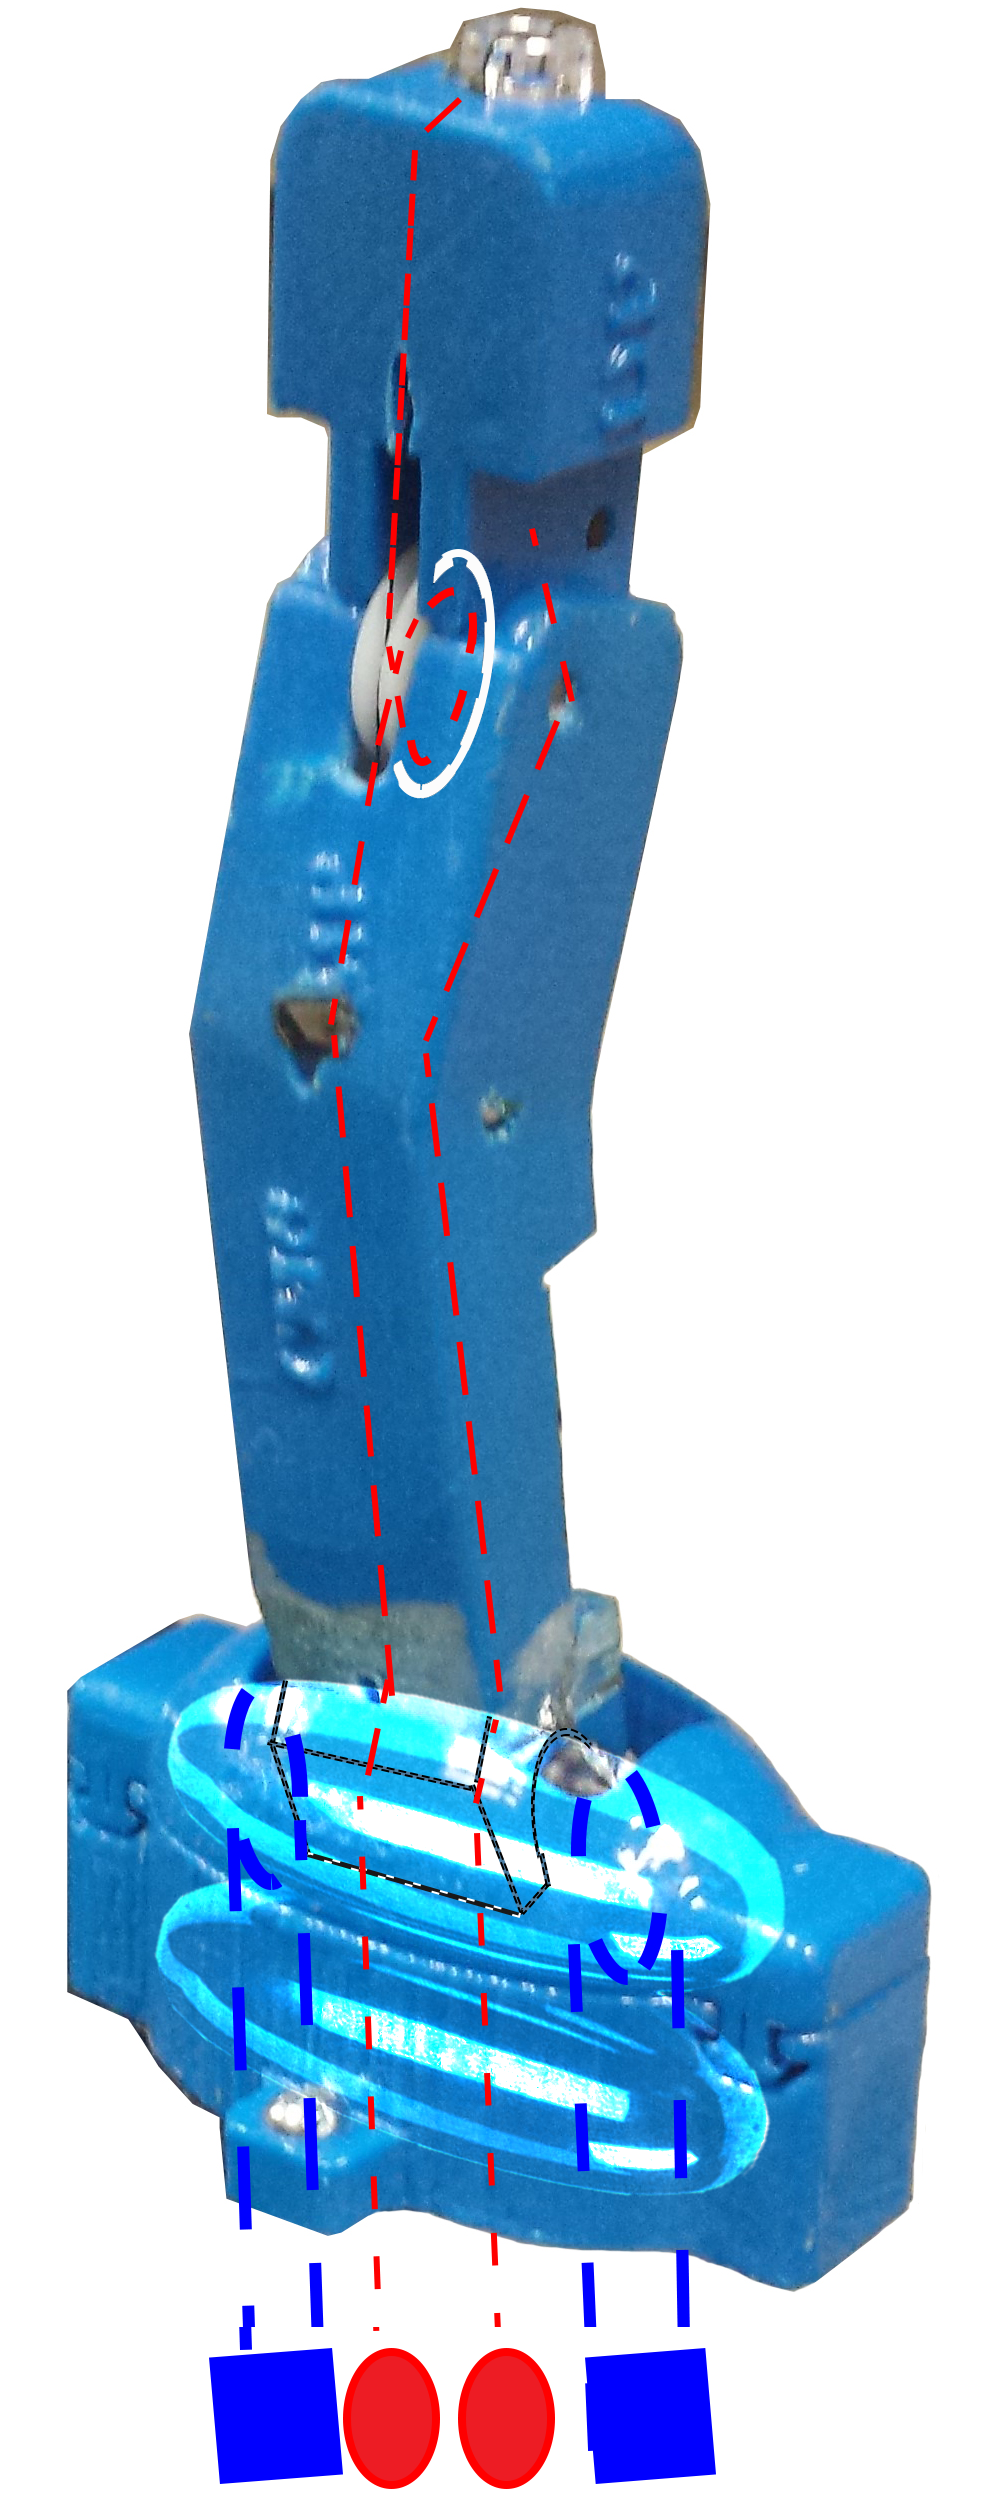
\includegraphics[width = 0.5\columnwidth]{thumb}
	\caption{Photograph of the prototype model. This prototype is based on the proposed Steiger arthrodesis at the metacarpal (MP) joint of the thumb, and also  and novel carpometacarpal (CMC) ellipsoidal joint. The locations of the interphalangeal (IP) joint and the ellipsoids of the CMC joint are highlighted in white and blue, respectively. The blue squares at the bottom represent single tendons that split around the elipsoids and terminate at the base of the metacarpal. From right to left, the blue tendons control adduction and abduction. The red tendons control flexion and extension, and terminate in the distal phalanx. To allow for underactuated grasping, the motion of the IP joint is mechanically coupled with that of the CMC joint. }\label{thumbphoto}
	\vspace{-15pt}
\end{figure}

The ACT hand is one example a very complex, biologically accurate hand design. One of the major obstacles to functionality is durability. Bow stringing, or the tendon traveling through free space, causes the ACT thumb's tendons to pull significantly far away from the digit as it comes under tension. Though it mimics human movement well, the tendons are easily damaged. Thus a design which houses the tendons within the structure is much more functional. Also along the lines of preserving functionality, high cost can prevent any device from reaching  the market. Keeping this in mind, the thumb presented here is designed to be 3D printed from ABS plastic, or any polymer filament available. Extruded ABS provides a strong, light, durable and very inexpensive structural material.

The biological human hand may still be superior, but it too is far from perfect. Are all of the anthropomorphic mechanics of the human thumb actually necessary, or even beneficial to modern use? What traits are mechanical remnants of forgotten tasks, or the remnants of evolutionary design? This paper focuses on the thumb, which provides a basal workspace for all the other digits to complete manipulative tasks within their own intersecting workspaces. By exploring new possibilities for modification to the first and second joints of the thumb, the CMC and the MP joints may be more closely imitated, or even improved upon.

\section{Tendon Routing Simplification}

By coupling the actions of multiple tendons and biological structures, it is possible to have access to all possible trajectories with discrete simplifications. As can be seen in \rFig{finger tendons}, our prototype thumb simplifies its tendon network into 4 tendons: one for adduction, abduction, flexion, and extension. Having four tendons arranged in this symmetric way allows for easy coordinate control and input.  There are 12 tendons which are connected in some way with the human thumb, and those which are used primarily for thumb manipulation are shown in /rFig{table1} \cite{grants anatomy}.

It is also with our device to simplify the tendons further: by coupling the hybrid extensor tendon $T_3$ with $T_1$ and $T_2$, then allowing that hybrid extensor tendon to also be coupled to the IP joint's extension, the two adduction/abduction tendons can be migrated to the extensor side. Distributing $T_3$'s load among formerly $T_1$ and $T_2$, $T_3$ is eliminated and a tripodal stability becomes possible, though harder to control. Also, this makes operation of the IP joint (when it is also under adduction or abduction) much more difficult, as the tendons must work against each other. This would significantly limit the grip strength of the thumb, while 4 tendons allow for much more efficient energy transmission during grasping, due to the radial location of each tendon with respect to the ellipsoids.

The choice was made to use a mechanical tendon and pulley system, instead of localized actuators. This further minimizes the complexity of the device by having as few actuators as possible. Not only does that improve the durability and weight, but it also reduces cost and is more biologically inspired than motors controlling each joint locally.

\begin{table}
	\centering
	\caption{Main tendons of the thumb simplified from 8 to 4}\label{tendonchoice}
	\begin{tabular}{c|c|c}
		Natural Tendon & Function & Replaced By \\
		\hline
		Abd. Pollicis longus & CMC Add. & $T_1$ \\
		Abd. Pollicis Brevis & Cmc Add. & $T_2$ \\
		Ext. Dorsal Expansion & MP Add./Abd., IP Ext. & $T_3$\\
		Ext. Pollicis Brevis & CMC Add. & $T_1$\\
		Oppenens Pollicis & CMC Flex. & $T_4$ \\
		Add. Pollicis & CMC Abduction & $T_2$ \\
		Ext. Pollicis Longus & CMC/MP Ext. & $T_3$\\
		CMC Joint Capsule & joint stability & Sliding Cap\\
		\hline
	\end{tabular}
\end{table}

\section{Consideration of Biological End Effectors}\label{concepts}

As the human thumb moves through its range of adduction/adduction motion, the CMC and MP joints adduct and abduct. The IP joint, even though it is a 1 Degree of Freedom pin joint, begins to abduct or adduct in reverse of the CMC and MP joints' adduction or abduction. The purpose of this is to ensure that the pulp of the thumb tip is always ready to engage in the hand's workspace. This functional coupling is a result of two other types of motion that are unique to the thumb: pronation and supination [cite]. This is significant to functionality, because the pulp of the thumb is its biological end effector. If the pulp did not rotate via pronation, grasping would be very difficult and unstable. This action happens mainly at the CMC joint [cite], and part of the role of the thumb's CMC sliding joint cap is to prevent this pronation by ensuring that the metacarpal cannot rotate relative to the base frame and base ellipsoid.

However, that instability is based on the assumption that the pulp of the thumb is restricted to a fractional hemisphere of the Distal Phalanx (DP). This is the case with the human hand, as our fingers must also accommodate the spacial needs of fingernails. By eliminating the nail and freeing up that space, the pulp can encompass the entirety of the distal phalanx, such that it will be ready to act into the shared workspace at any degree of flexion, extension, abduction or adduction; thus, there is no reason for the pronation of the thumb to be preserved in this device.

In terms of the pulp's overall gripping capability, the skin of the fingertip is highly detailed with ridges that assist us in gripping. While the 3D deposition process does leave somewhat similar ridges, they are not consistent or controllable in such a way as to improve the thumb's grip. An alternative process was used, known as acetone vapor finishing. ABS plastic is soluble in acetone, and when exposed to acetone gas in a closed container, it only takes a short period of time for the outer layers of material to become malleable. If the acetone is left too long, it may damage the structure, but can also create a much smoother and tackier surface than ABS printing alone. This acetone treatement leaves a gloss that seems to improve both the visual appeal of the ABS and gripping abilities when carefully applied to the distal phalanx.

The joint most distal from the base of the thumb, the IP, has only 1 Degree of freedom. However this range varies significantly among the population, with a significant amount of the human population being able to hyper extend the IP joint in a gesture known as the \emph{Hitchiker's Thumb}. Since this extreme range of motion is not required for any useful grasping purposes conceivable, it is not preserved. Our prototype's IP joint remains fundamentally unmodified from its biological equivalent, with an average joint range of 0 to 80 degrees [cite
 AAOS]. The MP and CMC joints of the human hand fill much more complex roles in grasping than the IP, but that does not mean they are the most important to functionality. In nature, each of these joints utilize a series of sliding joints that cannot be easily replicated in a mechanically constraining way. However, their contribution to overall thumb and hand functionality may be preservable, while still undergoing significant mechanical simplification.

\section{Arthrodesis of the Metacarpophalangeal Joint}\label{concepts}

From a robotics perspective, the preservation of an end effector's workspace is critical to its function, especially when that manipulator's function is interdependent on other manipulators who all share overlapping workspaces. In the field of orthopedic surgery, this problem has been recognized for many years. Arthritis, carpal tunnel, and other serious forms of thumb joint degeneration are very common, and often require fusion. When fusion of the MP joint is necessary, surgeons have found that overall hand functionality is best preserved, as opposed to fusion of the IP or CMC joints.

Arthrodesis is a well known procedure for patients with limited or exceedingly painful joint mobility to regain function through such a fusion. The damaged joint is fused with a series of metal screws and plates that permanently lock the joint into a specific set of angles. These fusions have been practiced on all three joints of the thumb, but with a notably high degree of functionality being preserved by MP joint fusions [cite steiger]. Through the heuristic process of many trials over many years, surgeons have refined a set angles of fusion that they deemed best for an MP thumb joint arthrodesis.

Two sets of angle parameters have emerged from these trials, specifically for the arthrodesis of the thumb's MP joint. The first model, proposed by Steiger, suggests that the MP joint be reduced from 2 Degrees of Freedom (DoF) to 0 DoF, a total fusion at 10 degrees of flexion and 15 degrees of abduction. Alternatively, the second model proposed by Wheeless suggests that the MP joint be allowed to retain motion about 1 DoF: thus, a limited range of 10 to 20 degrees flexion, and a fixed angle of 20 Degrees abduction [cite Wheeless]. These studies focus on identifying what works best for the treatment of damaged joints, rather than the applicability of the procedure as a robotic simplification. Using robotics methodology to explore the volumes and trajectories of these workspaces---relative to those of the natural thumb's workspace---helps to identify the positive and negative impacts of arthrodesis on a robotic thumb manipulator.

\begin{figure}
	\centering
	\subfloat[][Unfused workspace]{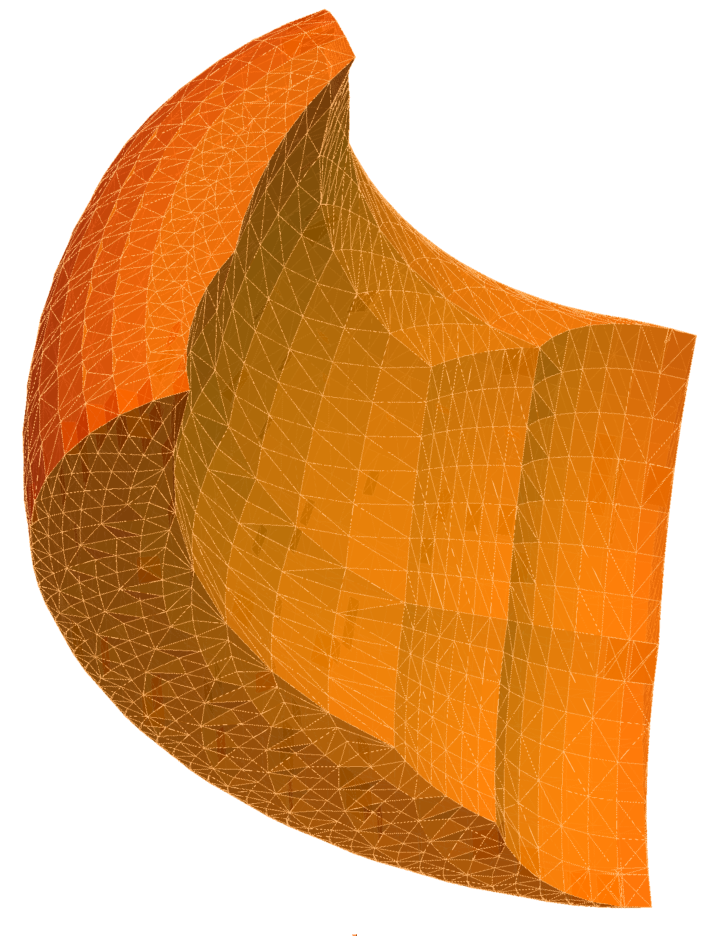
\includegraphics[width = 0.50\columnwidth]{Unfused}\label{schem}}\\
	\subfloat[][Steiger workspace]{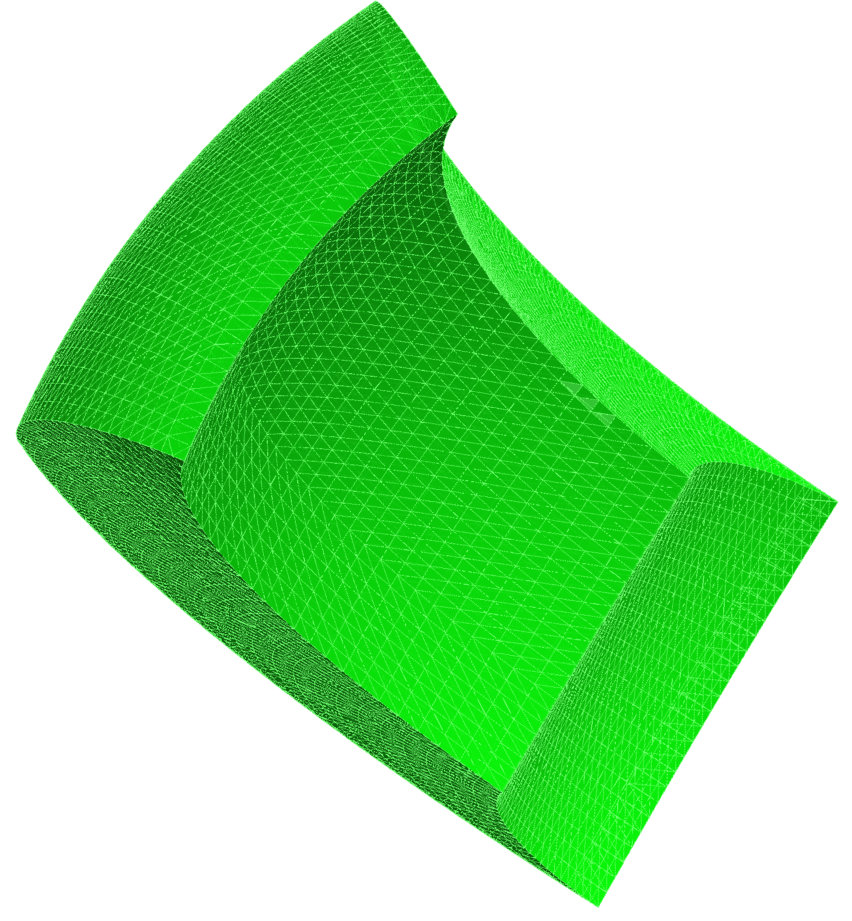
\includegraphics[width = 0.45\columnwidth]{Steiger}\label{contract}}%
	\subfloat[][Wheeless workspace]{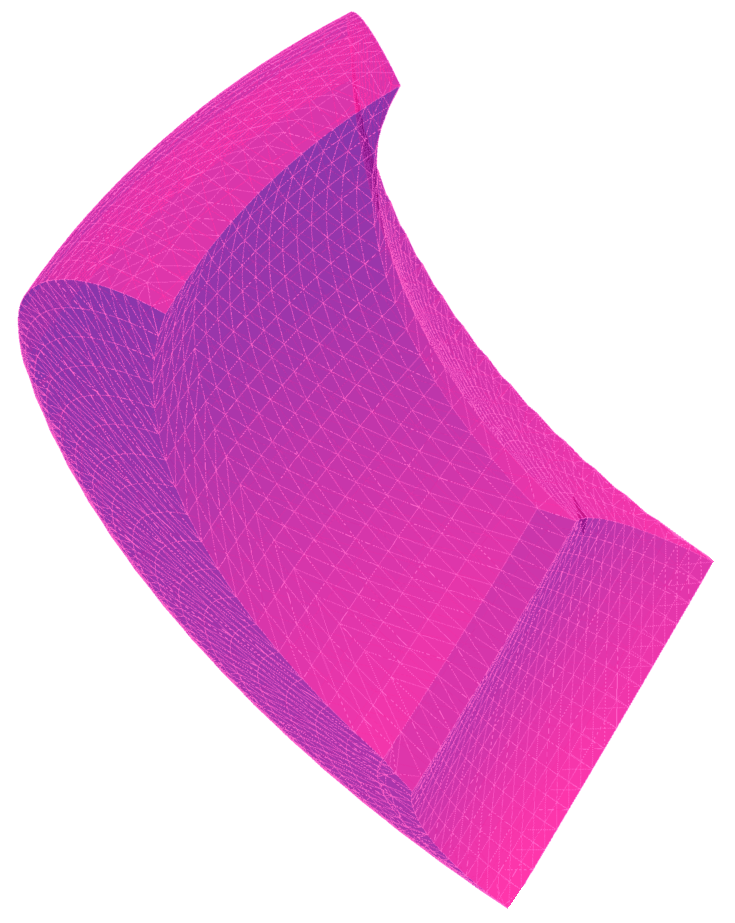
\includegraphics[width = 0.4\columnwidth]{Wheeless}\label{overload}}\\
	\subfloat[][Unfused, Wheeless and Steiger Workspaces]{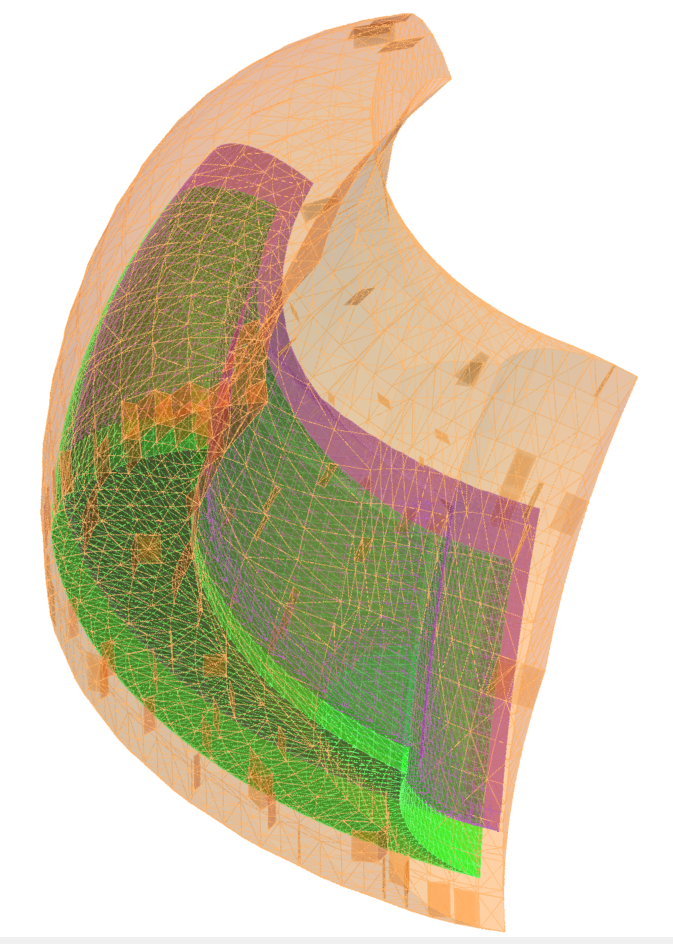
\includegraphics[width = 0.75\columnwidth]{Threespace}\label{old}}%
	\caption{Alternative Workspaces of our left handed thumb. The effect of the arthrodesis is seen immediately between (a) and (b), as (b) has around half the size of the unfused volume. Wheeless' and Steiger's parameters produce similarly shaped point clouds, with the main variation being the positioning within the unfused cloud. The Steiger fusion results in a marginally smaller volume than the Wheeless fusion; both fusions are about half the volume of the unfused workspace.}\label{workspaces}
\vspace{-6pt}
\end{figure}

To evaluate which of these arthrodesis parameters works better for an anthropomorphic hand, the volume and shaping of their resultant thumb workspaces can be overlaid in the same 3D space and visually inspected by comparing it to an identical but unfused thumb's workspace, as seen in \rFig{workspaces}.
	
	To generate these workspaces, Denavit Hartenberg Parameters (DH) were incorporated into a series of homogeneous transformation matrices, as shown in \rFig{dhtable}. The DH parameters serve as a conventionalized way to attach subsequent reference frames to one another for each link, creating a kinematic series of matrix multiplications. This chain represents the path of the thumb, where the angle constraints and lengths of the thumb segments are defined using robot manipulator notation. 
	
\begin{table}
	\centering
	\caption{Volumes of alternative thumb workspaces}\label{volumes}
	\begin{tabular}{c|c|c}
		Model Parameters & Volume (c$m^{3}$) & \% reduction \\
		\hline
		Unfused & 504.2 & \\
		Steiger & 207.1 & 58.9\% \\
		Wheeless & 223.5 & 55.7\% \\
		Prototype (Steiger) & 241.0 & 52.2\% \\
		\hline
	\end{tabular}
\end{table}	
	
When using DH convention, each matrix in a series represents a change of reference frame from one manipulator link to the next \cite{}. Thus to simulate the workspace volume, a function was written using \emph{Mathematica 10.1} to send a different combination of possible joint angles each time through the series of transformation matrices. The combinations were made to access every point in the workspace by using stepwise range functions, that discretize the range of motion into a set of unique joint angles. This resulted in a series of points in 3D space, which were correspondent to the position of the end effector when the thumb is at different combinations of joint angles. For both fusions and the unfused workspace, 3D point clouds were generated, representing the 3D workspace volume of that thumb model as shown in \rFig{workspaces}. The imputs used for the DH parameters of all workspace models are shown in \rFig{dhtable}.

\begin{table}
	\centering
	\caption{DH Parameters for transformatrion matrices $M_i$. The 4th input variable, $d_i$=0, is true for all matrices, representing translation along the $z_i$ axis. Angle measurements are shown in degrees, but are converted to and calculated as radians within the computation. All rotation happens counterclockwise relative to the axis of rotation. Link Lengths $\ell$ are defined at the bottom of the tabl,e and angle functions F$\rightarrow$I are found in /rEqn{1-5}.  The symbol $\leftrightarrow$ denotes a stepwise range function between the two extreme angle values.}\label{dhtable}
	\begin{tabular}{c|c|c|c}
	Input & & & \\
		Variable (IV) & $\alpha_{i-1}$ & $a_{i-1}$ & $\theta_i$ \\
		\hline
		Computational & & & \\
		 Order: & 1 & 2 & 3 \\
		Units: & (deg.) & (mm) & (deg.) \\
		IV Function: & Rot. $x_{i-1}$ axis  & Tran. $x_{i-1}$ axis & Rot. $z_i$ axis \\
		\hline
		Unfused M1 & 0 & 0 & 0$\leftrightarrow$70\\
		Unfused M2 & 90 & 0 & -15$\leftrightarrow$20 \\
		Unfused M3 & 0 & $\ell_{mcp}$ & -15$\leftrightarrow$15\\
		Unfused M4 & -90 & 0 & 0$\leftrightarrow$50 \\
		Unfused M5 & 0 & $\ell_{pp}$ & 0$\leftrightarrow$80 \\
		Unfused M6 & 0 & $\ell_{dp}$ & 0 \\
		\hline
		Steiger M1 & 0 & 0 & 0$\leftrightarrow$70 \\
		Steiger M2 & 90 & 0 & -15$\leftrightarrow$20 \\
		Steiger M3 & 0 & $\ell_{mcp}$ & 10 \\
		Steiger M4 & -90 & 0 & 15 \\
		Steiger M5 & 0 & $\ell_{pp}$ & 0$\leftrightarrow$80 \\
		Steiger M6 & 0 & $\ell_{dp}$ & 0 \\
		\hline
		Wheeless M1 & 0 & 0 & 0$\leftrightarrow$70 \\
		Wheeless M2 & 90 & 0 & -15$\leftrightarrow$20 \\
		Wheeless M3 & 0 & $\ell_{mcp}$ & 20 \\
		Wheeless M4 & -90 & 0 & 10$\leftrightarrow$20 \\
		Wheeless M5 & 0 & $\ell_{pp}$ & 0$\leftrightarrow$80 \\
		Wheeless M6 & 0 & $\ell_{dp}$ & 0 \\
		\hline
		Prototype M1 & 0 & 0 & -12.5$\leftrightarrow$12.5 \\
		Prototype M2 & 90 & 0 & -4.375$\leftrightarrow$4.375\\
		Prototype M3 & 0 & F($\theta_2$) & G($\theta_2$) \\
		Prototype M4 & 0 & F($\theta_2$) & H(($\theta_2$) \\
		Prototype M5 & -90 & $\ell_{mcp}$ & I(($\theta_1$) \\
		Prototype M6 & 90 & 0 & 10 \\
		Prototype M7 & -90 & $\ell_{pp}$ & 15 \\
		Prototype M8 & 0 & 0 & -11$\leftrightarrow$107.5 \\
		Prototype M9 & 0 & $\ell_{dp}$ & 0\\
		\hline
		\hline
	\end{tabular}
	\begin{tabular}{c|c|c}
	Structure & Variable & Length (mm) \\
	\hline
	Metacarpal & $\ell_{mcp}$ & 52.9 \\
	Proximal Phalanx & $\ell_{pp}$ & 40.3 \\
	Distal Phalanx & $\ell_{dp}$ & 30.7 \\
	Ellipsoid Major Radii & $R_{maj}$ & 21.02 \\
	Ellipsoid Minor Radii & $R_{maj}$ & 7.60 \\
	\hline
	\hline
	\end{tabular}
\end{table}

\begin{multline}
	F(\theta_2) = \\
	|\sqrt{R_{maj}^{2}/(1-\cos^{2}\theta_2+(R_{maj}/R_{min})^{2}*\cos^{2}\theta_2)}| 
	\end{multline}
\begin{multline}
	G(\theta_2) = \\
	2(\arctan((R_{min}/R_{maj})^{2}*\tan|\theta_2|)-|\theta_2|)*\sin(-\theta_2) 
	\end{multline}
	\vspace{-12pt}
	\begin{eqnarray}
	H(\theta_2) = \theta_2 \\
	I(\theta_1) = \theta_1 
\end{eqnarray}

\section{CMC Joint: Twin Prolate Ellipsoids}

\subsection{Mechanical Design Justification}

Mechanical Thumbs often use a pin joint, two pin joints coupled at perpendicular axes of rotation, or simply a joint with a series of locking positions to create the thumb's trajectory. This CMC joint represents a novel kind of joint that uses ellipsoidal magnets to approximate the conic rolling path taken by the natural thumb's metacarpal across its trapezium. 

The range of motion of the CMC has been defined many different ways, with significant disagreement on how to characterize the rolling of the metacarpal across the highly irregular surface of the trapezium \cite{Hollister}. One of the reasons for this is that the CMC does not fit neatly into a  standard joint type, not does it lend itself to being reduced to a system of traditional joints. Rather, it is best modeled as a complex surface joint \cite{Synek}. Previous research \cite{Chalon} suggests the use of an ellipsoidal surface joint is the best way to to mimic the rolling/gliding motion of the CMC joint complex. 

To accommodate this joint's large range of motion when unbounded, mechanical limits were established by creating an encasement around the CMC joint. The joint occurs at the mutual contact point of the two ellipsoids, in the middle of the joint housing. The sliding cap is sets mechanical limits (via the dimensions of it's opening for the metacarpal, and the range of its sliding motion) for flexion/extension and adduction abduction. 

\begin{figure}
	\centering
	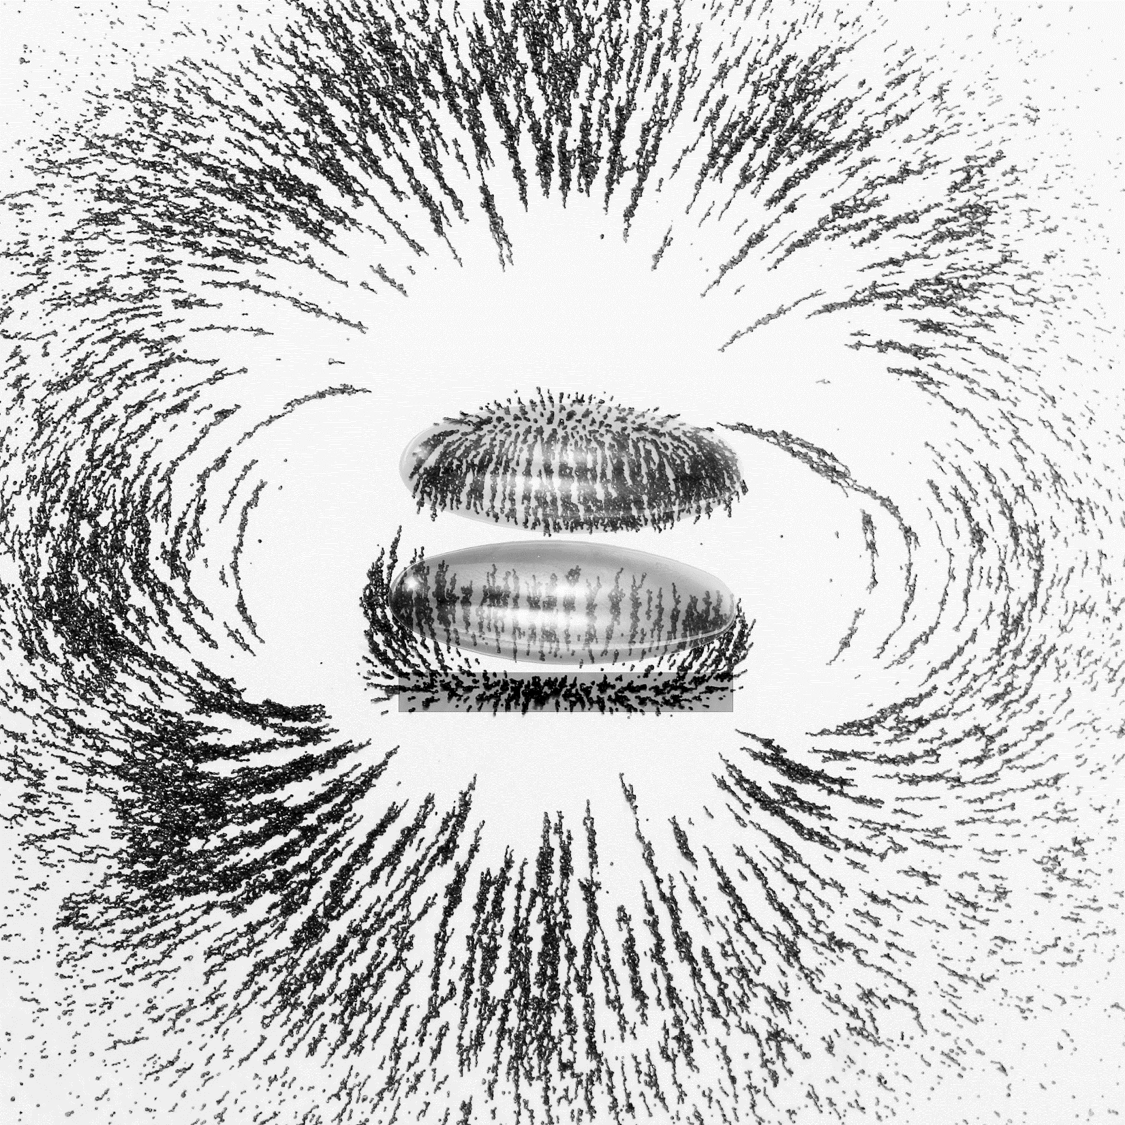
\includegraphics[width = 1\columnwidth]{magnets}
	\caption{The magnetic forces at play in the CMC joint can be examined more closely by using iron filings, and a white boundary for the ellipsoids and plate to sit behind. Images of the ellipsoids and plate have been superimposed over this photograph. The ellipsoids' magnetic fields run perpindicular to their major axes, causing the magnets to be most stable when placede side by side. The effect of the ferros plate is seen directly below the bottom elipsoid, with which it is in direct contact with: along the plane of the plate, an array of vertical lines intersect the page. These field lines coming from the plate are coplanar with the ferrous plate, showing that it is redirecting more field lines to flow coplanar to itself, and perpendicular to the normal axis of the thumb itself. As the poles are colinear with the normal axis when at rest, the plate thus creates a subtle joint force which functions as a way to stabilize the resting position of the thumb, and to ensure that the resting position will be less likely to become displaced during movement.}\label{magnet}
	\vspace{-15pt}
\end{figure}


\begin{figure}
	\centering
	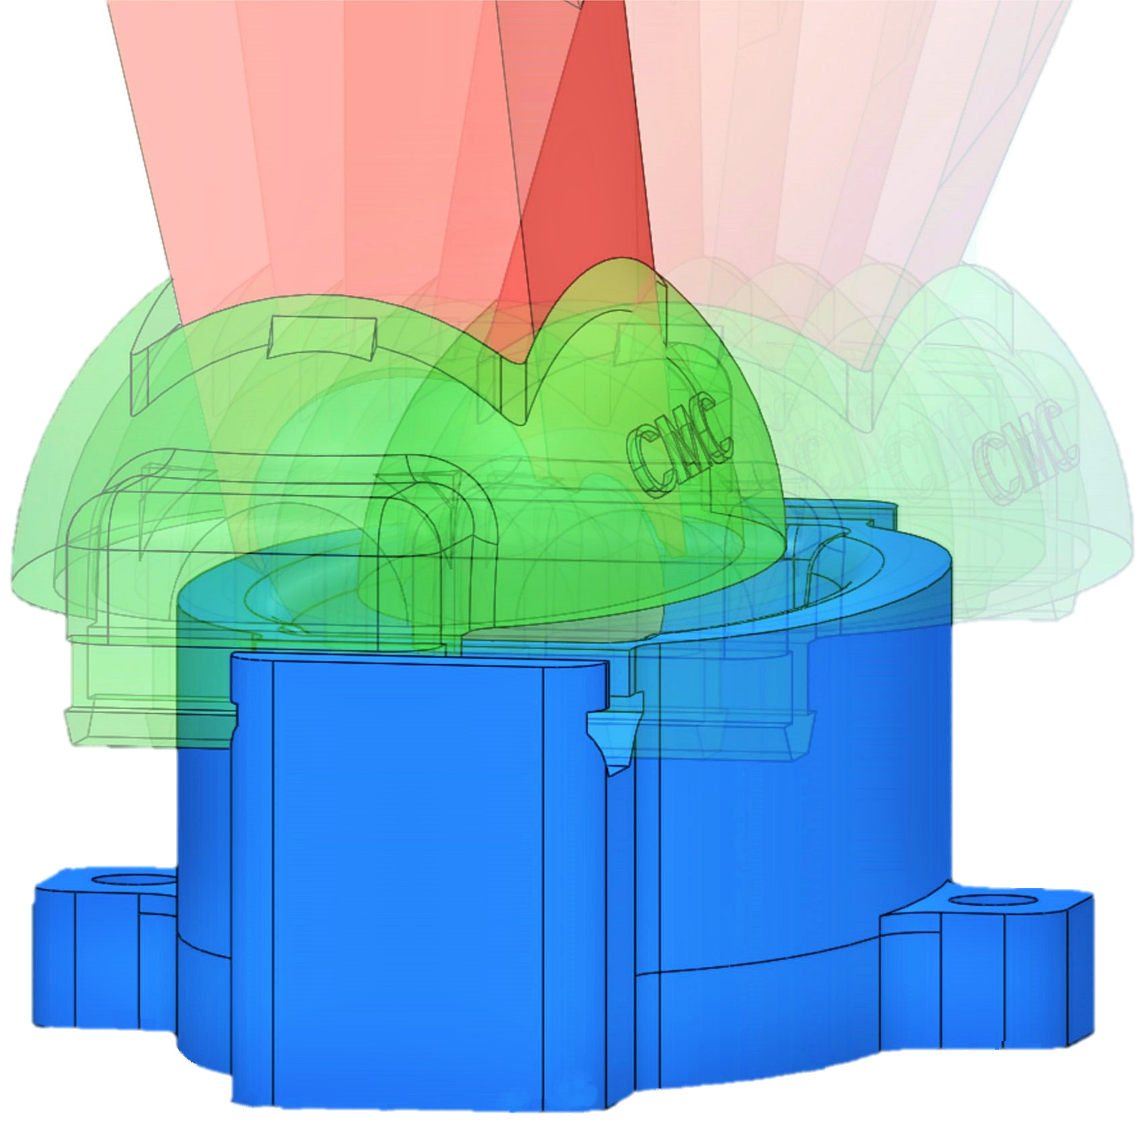
\includegraphics[width = 1\columnwidth]{cmcgraphic}
	\caption{This CAD representation shows the CMC joint following a linear trajectory across both ranges of motion. On the left, The CMC joint is seen tracing a linear trajectory from its maximally adducted and extended position to its maximally abducted and flexed position. The bottom of the CMC joint is shown in blue, and the base plane is approximately coplanar with the plane of the palm of the hand. The CMC embossment faces inward, toward the combined workspace of the thumb and fingers. The metacarpal interphalanx fusion, in red, is prevented from twisting along its own axis by the CMC cap, in green. As intended, this stabilizes the joint by restricting it to only 2 Degrees of freedom instead of the natural thumb's 3 Degrees of freedom.}\label{cmcgraphi}
	\vspace{-15pt}
\end{figure}

\subsection{Choice of Ellipsoids}

Ellipsoids, as spheroids, share a fundamental property: when one is rolling in rotation around another, it rotates along its own axis twice as rapidly, in terms of angular deflection from the vertical resting position. This means that the metacarpal needs to roll only half as far as it would on a flat surface to generate an equivalent amount of rotation about itself. This results in a significant decrease in the overall size of the joint housing. Because of this, the concept of twin ellipsoids seems to be the most compact way to utilize the concept for a thumb joint.

The search criteria for a suitable ellipsoidal base focused on functionality, but as the goal was to minimize cost of materials and manufacturing, only consumer ready products were considered. Each "Egg" is has no obvious surface discrepancies, but as they are intended to be used as novelty products (as the magnets mimic a rattlesnake noise when thrown together) their curvature is only roughly ellipsoidal. However, they are also powerful magnets whose magnetic poles run perpendicular to their major axis, meaning that they are most stable magnetically when side by side, as shown in \rFig[thumb]. The chosen ellipsoids are also prolate, which allows for greater range of motion when the trajectory is along the minor radii of the ellipsoids. Thus, as shown in \rFig[thumb], the minor radial discs of the ellipsoids are coplanar with the flexion/extension axis of the metacarpal. The major axis of the ellipsoids is perpendicular to this, inhabiting the plane of CMC adduction/abduction motion. 

\subsection{CMC Joint Limits: Magnetic and Mechanical}

To build the CMC joint limits, one of the ellipsoids is inserted into the bottom of the ABS joint housing, and secured in place with a small elliptical plate of steel. This plate is ferrous, and interacts in a beneficial way with the ellipsoids, as it creates a third point of attraction directly below the first two, ensuring that the elipsoids' magnetic poles point straight upwards from the sheet steel.

As the steel plate also defines the base plane of the thumb's first reference frame, this means that the most stable point for the finger is in colinearity with the base's normal vector. The magnetic forces causing this effect can be seen in the linear concentration of iron filings along the plane of the sheet steel in /rFig{magnet}. This also means that the magnetic joint forces cause the thumb to return to its neutral position spontaneously even if the bottom ellipsoid begins to rotate or shift. Magnetic interaction creates partial joint forces help hold the thumb together passively, so that under extreme duress it can come free without structural failure, but under normal usage will not jam or become out of line.

\subsection{Prototype Durability}

The second ellipsoid is secured to the metacarpal with an adhesive, in a position where the metacarpal is parallel to the ellipsoid's major axis and colinear with the magnetic poles aligned below it. This position is referred to as the thumb's resting position, due to the stability created by the magnetic fields. As part of the metacarpal, the top ellipsoid will rotate around and over the base ellipsoid, which remains fixed. This motion is meant to closely mimic that of a natural CMC joint. But like their natural equivalents, ellipsoidal surface joints are still relatively fragile. The solution to this lies in the CMC's use of a sliding cap.

If a high enough tensile load is applied to the thumb, the magnetic attraction will be overwhelmed and will release, but the CMC joint will initially stay intact because of the sliding cap. The cap also prevents dislocation under load: though the ellipsoids may slide over each other if forced, a gripping or weight bearing load will only be able to slightly deflect the joint before being locked into position by the sliding cap and joint base.

 In the case of an even greater force, the CMC joint will be able to dislocate to prevent structural damage, as the opening in the sliding cap has an inside channel cut into it near the opening that allows it to flex just enough to allow dislocation. The tendons would be damaged by such an event, but are easily replaceable. Without the sliding cap, the prevention of dislocation would rest solely on the magnetic forces highlighted in \rFig{magnet}.
 
  The sliding joints of the cap are lubricated using graphite powder to prevent jamming, another source of acute damage. Jamming of the sliding joint would not be an issue if the joint were made out of a harder material than ABS, which also reduces the joint's resistance to flexion and extension.

\subsection{CMC Tendon Routing}

As seen in \rFig{thumbphoto}, flexion/extension of the CMC is coupled to the IP joint, to allow underactuated grasping motions, which is an important characteristic of anthropomorphic hands \cite{Martell}. Abduction/Adduction tendons travel through holes in the plate and base, then terminate within the CMC joint, respectively secured to the mobile ellipsoid's prolate poles. These tendons do not need to extend further along the finger, as the MCP fusion means that there is no need for abduction/adduction further down the digit, as shown in \rFig{thumbphoto}. The remaining two tendons travel up to the distal phalanx, coupling IP and CMC flexion/extension.

\section{CMC Ellipsoid Joint Workspace Simulation}

In \rFig{dhtable}, the matrices used for the calculation of the prototype's workspace are defined, based on DH parameters and conventions. As the CMC joint does not represent a constant link length or angle, new functions had to be introduced in the extra matrices to step through the joint using virtual linkages. The first and second linkages mirror each other about the tangent plane shared by the ellipsoids at their point of contact. These linkage lengths are a function of the radial distance from the center of the ellipsoid to its surface, which itself is a function of $\theta_1$ and $\theta_2$. In \rFig{dhtable}, this function is represented by F($\theta_2$). The internal angle between these two linkages at the junction is determined as a function of the slope of the tangent plain of the ellipsoid, seen in function G($\theta_2$) in \rFig{dhtable}. As mentioned, the rotation's self doubling action of two ellipsoids defines the next transformation into the frame of the metacarpal. From there on, the matrices follow those of the Steiger arthrodesis workspace. This workspace was chosen for the overall thumb because of its simplicity, and because of its comparability with the more complicated Wheeless workspace.

A limitation of this  computation is that it does not account for the CMC joint's nonholonomic nature; that is, as a rolling surface joint, its joint constraint equations are also dependent on nonintergrable functions of the dependent velocity \cite{Springer}. This would mean that assuming a no slip condition, the joint will not necessarily return to its rest position using DH parameters, and could end up somewhere else. This blurs the definition of the workspace, since some areas outside the calculated workspace may also be accessible under certain velocities.

That being said, there are two reasons that it may still function as a holonomic joint. First, the sliding cap limits rotation of the metacarpal to nearly zero, suggesting that the DoF requirements to be a nonholonic joint are not met. Second, the joint's magnetic forces also reset position and rotation of the metacarpal to zero whenever the thumb is at rest. Future work will explore this possible problem further, by applying different equation sets that are more suited to both holonomic and nonholomic joints, such as the Boltzmann Hamel Equations \cite{Cameron}.

\begin{figure}
	\centering
	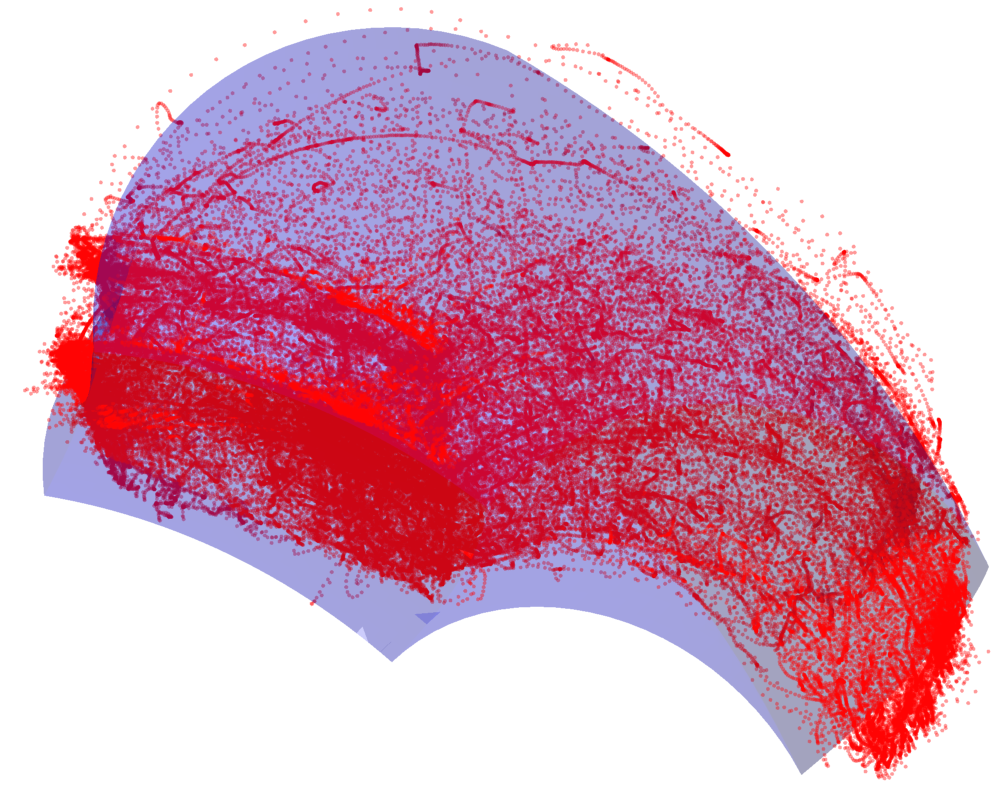
\includegraphics[width = 1\columnwidth]{data}
	\caption{The red points were recorded from the prototype, plotted simultaneously with the simulated workspace of the prototype, which appears as a blue volume.}\label{dat}
	\vspace{-15pt}
\end{figure}

\section{Experimental Results}

One of the major limitations of the prototype is that the sliding cap's mechanical joint limits were  too restrictive along some ranges of motion. The CMC flexion/extension range was reduced from $70^{\circ}$ to $52^{\circ}$, a decrease of \%26. The adduction/adduction range was more accurate, allowing $38^{\circ}$ instead of $35^{\circ}$, an increase of \%9.

On the other end of the spectrum, the prototype's IP joint is hyper flexible (most likely due to the ABS deforming from requent use) with a range of $-11^{\circ}$ to $107^{\circ}$ degrees, representing a \%47 increase. Yet this is not outside normal IP joint range for many individuals. Future research is needed to determine the impact of IP hyper flexibility on thumb functionality.

Using electromagnetic motion capture sensors, the point cloud data in \rFig{dat} was gathered using a electromagnetic motion tracking instrument, at a rate of 240 Hz. 10 trials were run over a period of 1 minute each, generating 143,796 data points all together. After duplicate points were removed, the point cloud was compared with the theorized workspace. 

From the right side of the figure, it is clear that a premature range of motion limit was being stopped at frequently, as seen in the two bands of red points. This is most likely due to occasional jamming of the CMC sliding cap that would occur as the thumb was brought from full extension to full flexion, causing the tip of the thumb to trace out the internal limit. This can be addressed by finding a better lubricant for the sliding joint, or finding a building material less prone to flexing and jamming, which was the main downside of using ABS. 

In general, the simulated workspace fits the the experimental data fairly well, suggesting that the transformations are describing the prototype accurately. A better measurement of this would be to measure the volume of the point cloud, but due to the number of internal points, there is no general algorith for the extraction of a valid surface. Other methods may prove more successful: for future research, a voxxel-based binning method as employed here \cite{Bullock} may produce better results.

The success of Steiger's surgical heuristics suggests that the workspace generated by his parameters provides sufficient thumb functionality. The workspace volume of the prototype, shown in \rFig{volume}, exceeds the Steiger workspace's volume by 16.4\%. When looking at volume and shape as indicators of workspace functionality, the prototype exceeds Steiger's volume, though it is of a slightly compressed shape due to the tight joint range limits of the CMC. Future research involving a refined prototype could explore this predicted functionality using grasping tests for the thumb in various couplings with other finger manipulators. 

\section{CONCLUSIONS}

In this paper, novel designs for the CMC and MP joints were explored, one a simplification, and the other an ellipsoidal surface joint. Through this process, a prototype thumb was developed which focuses on maximizing durability and functionality, while minimizing cost and unnecessary complexity. Heuristic joint parameters \cite{Steiger} were applied to the MP joint of the prototype to determine a possibly beneficial joint fusion, surgically known as Steiger arthrodesis. While this arthrodesis did not provide the largest workspace volume initially, the prototype was ultimately built with it to maximize strength and simplicity.

The Steiger prototype's volume was the largest volume of all fusions analyzed, suggesting high thumb functionality. These workspaces were generated using Denavit Hartenberg parameters to determine the path of the thumb through many workspaces under many different constraints. Future work will refine the design of the prototype and the workspace simulation, investigating both design improvements to more accurately reflect the range of motion of the CMC joint, and evaluating the applicability of nonholonomic equations for modeling twin ellipsoidal joints. 

%\addtolength{\textheight}{-12cm}   % This command serves to balance the column lengths
                                  % on the last page of the document manually. It shortens
                                  % the textheight of the last page by a suitable amount.
                                  % This command does not take effect until the next page
                                  % so it should come on the page before the last. Make
                                  % sure that you do not shorten the textheight too much.

%%%%%%%%%%%%%%%%%%%%%%%%%%%%%%%%%%%%%%%%%%%%%%%%%%%%%%%%%%%%%%%%%%%%%%%%%%%%%%%%

%\listoftodos

%%%%%%%%%%%%%%%%%%%%%%%%%%%%%%%%%%%%%%%%%%%%%%%%%%%%%%%%%%%%%%%%%%%%%%%%%%%%%%%% 



%%%%%%%%%%%%%%%%%%%%%%%%%%%%%%%%%%%%%%%%%%%%%%%%%%%%%%%%%%%%%%%%%%%%%%%%%%%%%%%%
%\section*{APPENDIX}
%
%Appendixes should appear before the acknowledgment.

%\section*{ACKNOWLEDGMENT}

%\printbibliography{biorob2014}
%\vspace{800pt}

\section{References}

\bibliography{biorob2014.bib}


\end{document}
